\section{Fun with Recurrences}

Give an asymptotic solution (which should be a $\Theta$-bound) to each of the recurrences below. You may use whatever solution method you wish (drawing out the tree, unrolling the recurrence, proof by induction, Master Theorem, etc.), but make sure you fully justify your answer.

\begin{questions}
	\question[3] $T(n) = 2T(n-1) + 1$ for $n > 1$, $T(1) = 1$.

	\ifsolutions\begin{soln}
	Claim: that
\end{soln}
\fi
	\begin{soln}
		\begin{align*}
			T(n) & = 2T(n-1) + 1                                    \\
			     & = 2(2T(n-2) + 1) + 1                             \\
			     & = 2^2T(n-2) + 2^1 + 2^0                          \\
			     & = 2^3T(n-3) + 2^2 + 2^1 + 2^0                    \\
			     & \dots                                            \\
			     & =2^{n-1}T(1) + 2^{n-2} + \dots + 2^2 + 2^1 + 2^0
		\end{align*}

		So my claim is, \(T(n) = \sum_{i = 0}^{n-1} 2^i = \frac{2^{n-1 + 1} - 1}{2 -1 } = 2^n - 1, n >1\).

		Proof: \(T(2) = 2T(1) + 1 = 3 = 2^2 - 1\). Base case holds. Then \(T(n+1) = 2T(n) + 1 = 2(2^n - 1) + 1 = 2^{n+1} - 1\). Thus, induction makes it hold.

		Then, \(\frac{2^{n}}{2} = 2^n - \frac{2^n}{2} \leq 2^n - 1 = T(n) \leq 2^n\). Hence, \(T(n) \in \Theta(2^n)\).
	\end{soln}

	\question[3] $T(n) = 3T\left( \frac{n}{2} \right) + e^n$ for $n > 1$, $T(1) = 1$.

	\ifsolutions\begin{soln}
	Let \(P = (v_1, v_2, \dots, v_n)\) be a permutation on \(V\).

	We will assume that we have an adjency matrix to represent the edges in the graph \(M\).

	\begin{algorithmic}[1]
		\Procedure {Valid-Ranking}{P, M}
		\For{each $i = 1, 2, \dots, n - 1$}
		\State store the sum from $j = i$ to $j = n$ of $M(j)$ as $d_i$
		\For{each $j = i + 1, \dots, n - 1$}
		\State store the sum from $k = j$ to $k = n$ of $M(k)$ as $d_k$
		\If{$d_i < d_k$}
		\State end the procedure, report it is not valid
		\EndIf
		\EndFor
		\EndFor
		\State report the permutation as valid
		\EndProcedure
	\end{algorithmic}
	This algorithm is \(O(n^3)\), where \(n = |P|\). In the worse case, we have a valid permutation, and the algorithm does work as follows.

	We have to iterate through the permutation list \(n - 1\) times. Access to the elements will be \(O(1)\) as we assume we are given an array.

	Then for each iteration, we are iterating through the entire adjency matrix, except each iteration we are considering one less node.

	Access to the adjency matrix is \(O(1)\) thus the iteration of the adjency matrix is \(O(i^2)\).

	Then, for each \(i\), the work we are doing is \(i^2\). Thus, summing \(i = 1, 2, \dots, n - 1\) gives us \(O(n^3)\).


\end{soln}
\fi
	\begin{soln}
		For the \(0\)th level of the tree, we are doing \(e^n\) amount of work then in the second we are getting, \(3e^{\frac{n}{2}}\).

		For any level of the tree we are going to be doing \(3^i e^\frac{n}{2^i}\) work. The height of the tree is \(\lg(n)\).

		Hence, \(T(n) = \sum_{i=0}^{\lg(n)} 3^i e^{\frac{n}{2^i}}\) for \(n > 1\). Then, if we consider \(\frac{T(n)}{e^n}\) we get:
		\[
			\frac{T(n)}{e^n} = \sum_{i=0}^{\lg(n)}3^i e^{n\left(\frac{1 - 2^i}{2^i}\right)} = 1 + 3e^{\frac{-n}{2}} + 3^2e^{\frac{-3n}{4}} + \dots + 3^{\lg(n)}e^{1-n}.
		\]

		Now, observe that if \(i \geq 1\) we get \(2^i \geq 2 \implies 1 - 2^i \leq -1 < 0\), since \(n > 1\) then \(1 - n < 0\).

		Hence, every term after \(i = 1\) has \(e^{-an}\) for some \(a > 0\) in other words, it decays exponentially.

		Then,
		\[
			\lim_{n \to \infty} \frac{T(n)}{e^n} = \lim_{n \to \infty} 1 + 3e^{\frac{-n}{2}} + 3^2e^{\frac{-3n}{4}} + \dots + 3^{\lg(n)}e^{1-n} = 1.
		\]

		Thus, \(T(n) \in \Theta (e^n)\).

	\end{soln}

	\question[3] $T(n) = T\left( \frac{n}{4} \right) + 2T\left( \frac{n}{16} \right) + \sqrt{n}$ for $n > 16$, $T(n) = 1$ for $n \le 16$.

	\ifsolutions\begin{soln}
	Suppose we are given a tournament graph \(T = (V, E)\) with a vertex ordering \(v_1, v_2, \dots, v_n\) such that for all \(i < j\), the directed edge \((v_i, v_j)\) is in \(E\). That is, every vertex points to all vertices that come after it in the order.

	\textbf{Claim 1:} \(T\) is a tournament.

	For every distinct pair \(v_i, v_j\), either \(i < j\) or \(j < i\), so exactly one of \((v_i, v_j)\) or \((v_j, v_i)\) exists in \(E\), but not both. This satisfies the definition of a tournament: for every pair of distinct vertices, there is exactly one directed edge between them.

	\textbf{Claim 2:} The ordering \(v_1, v_2, \dots, v_n\) is a valid ranking.

	Let \(d_i\) be the out-degree of \(v_i\) in the subtournament induced by \(\{v_i, v_{i+1}, \dots, v_n\}\). Since \(v_i\) points to all vertices that follow it, it has out-degree \(d_i = n - i\). For \(i < j\), \(d_i = n - i > n - j = d_j\), so each player has strictly higher out-degree than those who come after them. Thus, the ordering satisfies the requirement of a valid ranking.

	\textbf{Claim 3:} The valid ranking is unique.

	Suppose for contradiction there is another valid ranking \(P' = v_{\pi(1)}, v_{\pi(2)}, \dots, v_{\pi(n)}\) with \(\pi\) a permutation of \(\{1, \dots, n\}\), and \(P' \ne P\). Then there exist indices \(i < j\) such that \(\pi(i) > \pi(j)\); that is, \(v_{\pi(i)}\) appears before \(v_{\pi(j)}\) in \(P'\), but comes later in the original ordering.

	But then in the subtournament starting at \(v_{\pi(i)}\), the vertex \(v_{\pi(i)}\) must have lower out-degree than \(v_{\pi(j)}\), contradicting the assumption that \(P'\) is a valid ranking. So the valid ranking must be unique.

	Suppose we have a tournament graph \(T = (V, E)\) such that there is an ordering, \(v_1, v_2, \dots, v_n\) so that there is an edge \((v_i, v_j)\) iff \(i < j\).

	This would create one valid ranking, and this ordering is exactly that ranking.

	Before we prove that statement, we will show it is a tournament in the first place, and that is is valid ranking.

	First, we require that every player has played someone else and only once or in other words, either \((v_i, v_j) \in E\) or \((v_j, v_i) \in E\) but not both.

	Let \(v_i, v_j \in V\) such that \(i \neq j\). Then either \(i < j\) or \(j < i\). Then we can only have one of the edge pairs in \(E\) by assumption.

	Next, we require that \(v_i\) has maximum out-degree in its subtournaments.

	Observe that for any \(v_i\) in a subtournament it's out degree is \(d_i = n - i + 1\), independent of the sub tournament.

	Then for any \(i < j\), we see that \(n - j + 1 < n - i + 1\), but this precisely means that \(d_j < d_i\), thus it is valid ranking.

	Proof: For contradiction, suppose that there were two valid rankings.

	Then it must be some permutation on \(P:= v_1, v_2, \dots, v_n\).

	Then there exists some \(i < j\) in \(P\) such that \(j < i\) in \(P'\). But this means that \(d_j < d_i\) in the subtournament for \(j\) in \(P'\).

	This contradicts that \(P'\) was a valid ranking.
\end{soln}
\fi
	\begin{soln}
		By drawing out the first three levels of the tree and its work needed to perform the subproblem, we see that:

		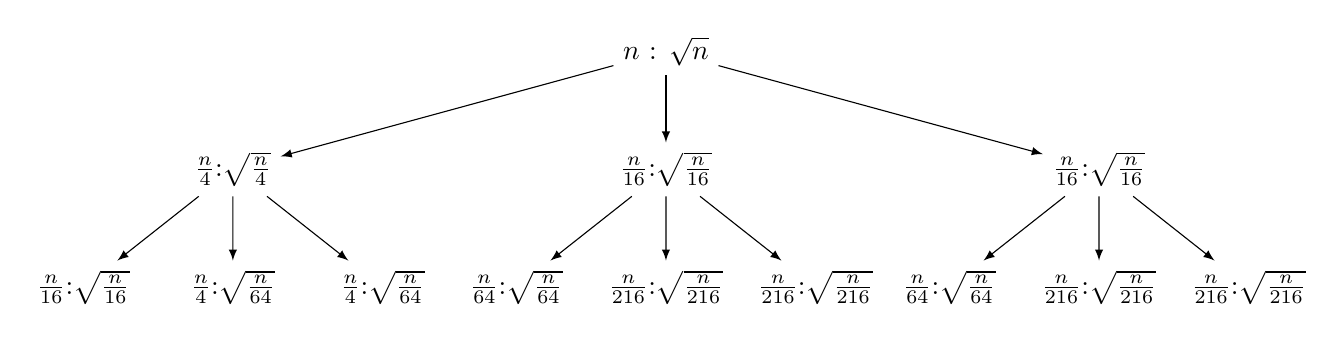
\begin{tikzpicture}[
				level 1/.style={sibling distance=55mm},
				level 2/.style={sibling distance=19mm},
				level 3/.style={sibling distance=10mm},
				edge from parent/.style={draw, -latex}
			]
			\node {\(n\) : \(\sqrt{n}\)}
			child {node {\(\frac{n}{4}\):\(\sqrt{\frac{n}{4}}\)}
					child {node {\(\frac{n}{16}\):\(\sqrt{\frac{n}{16}}\)}}
					child {node {\(\frac{n}{4}\):\(\sqrt{\frac{n}{64}}\)}}
					child {node {\(\frac{n}{4}\):\(\sqrt{\frac{n}{64}}\)}}
				}
			child {node {\(\frac{n}{16}\):\(\sqrt{\frac{n}{16}}\)}
					child {node {\(\frac{n}{64}\):\(\sqrt{\frac{n}{64}}\)}}
					child {node {\(\frac{n}{216}\):\(\sqrt{\frac{n}{216}}\)}}
					child {node {\(\frac{n}{216}\):\(\sqrt{\frac{n}{216}}\)}}
				}
			child {node {\(\frac{n}{16}\):\(\sqrt{\frac{n}{16}}\)}
					child {node {\(\frac{n}{64}\):\(\sqrt{\frac{n}{64}}\)}}
					child {node {\(\frac{n}{216}\):\(\sqrt{\frac{n}{216}}\)}}
					child {node {\(\frac{n}{216}\):\(\sqrt{\frac{n}{216}}\)}}
				};
		\end{tikzpicture}



		If the top is level \(0\), then we see at level \(1\) we are doing \(\sqrt{n} \cdot ( \frac{1}{2} + \frac{1}{4} + \frac{1}{4}) = \sqrt{n}\) amount of work.

		At level \(2\), we are again doing \(\sqrt{n} \cdot (\frac{1}{4} + \frac{1}{8} + \frac{1}{8} + \frac{1}{8} + \frac{1}{16} + \frac{1}{16} + \frac{1}{8} + \frac{1}{16} + \frac{1}{16}) = \sqrt{n}\) amount of work.

		Then for each level \(i\) we are doing \(\sqrt{n}\) amount of work, then we have that \(h = \log_{16}(n)\) is the amount of levels we have to work through.

		Thus, \(T(n) = \log_{16}(n) \cdot \sqrt{n} \in \Theta (\sqrt{n} \log(n))\).
	\end{soln}

	\question[3] $T(m,n) = mT(m, \frac{n}{3}) + n$ for $m \ge 1$ and $n \ge 3$; $T(m,n) = 1$ for $m \ge 1$ and $n < 3$.

	\ifsolutions\begin{soln}
	Find the set \(S_0\) such that each node in \(S_0\) has equal out-degree and is the greatest amongst all \(V\).

	Find the set \(S_1\) such that each node in \(S_1\) has equal out-degree and is the greatest amongst all \(V \setminus S_0\).

	Find set \(S_k\) so that each node in \(S_k\) has equal out-degree and is the greatest amongst all \(V \setminus \bigcup_{i=0}^{k-1}S_i\).

	Continue until you have a collection, such that \(\bigcup_{i = 0}^{k} S_i = V\).

	Then create a set of permutation, \(P_0, P_1, \dots, P_k\) such that \(P_i\) contains all possible permuations of ordered tuplets on vertices in \(S_i\).

	Next, create another set containing all ordered tuples of \(r = (p_1, p_2, \dots, p_k)\) where each \(p_i \in P_i\).

	Return \(R = \{\text{all possible } r\}\) as the set all possible valid rankings.

\end{soln}
\fi

	\begin{soln}
		We consider cases on a fixed \(m\). Once \(m\) is chosen, it remains the same for every recursive call.

		We will show that each case corresponds to a certain case of the master thoerem, denote \(f(n) = n\).

		Case \(m > 3\), then \(\log_3(m) > 1\). Then set \(\varepsilon = \log_3(m) - 1 > 0\) so that \(\log_3(m) - \varepsilon = 1\).

		Thus, \(f(n) \in O(n^{\log_3(m) - \varepsilon})\). This corresponds to case \(1\) theorem, thus \(T(n) \in \Theta(n^{\log_3(m)})\).

		Case \(m = 3\). Then \(\log_3(m) = 1\). We see that \(f(n) = n \in \Theta(n^{\log_3(m)} \log^0(n))\).

		This corresponds to case 2 of the master theorem. Hence \(T(m, n) \in \Theta (n \log(n))\).

		Case \(m \leq 2\). Then \(0 < \log_3(m) < 1\), and hence we can set \(\varepsilon = 1 - \log_3(m) > 0\) so that \(\varepsilon + \log_3(m) = 1\).

		Then we see that \(n \in \Omega(n^{1+\varepsilon})\). Then observe that \(m < 3 \implies \frac{m}{3} < 1 \).

		Now, take any \(\delta\), with \(0 < \frac{m}{3} < \delta < 1\) so that \(m f(\frac{n}{3}) = \frac{mn}{3} < \delta n = \delta f(n)\).

		This corresonds to case \(3\) of the master theorem, thus \(T(m, n) \in \Theta (n)\).

	\end{soln}


\end{questions}
